\section{Monte Carlo Intervention Results}\label{sec:results}

The confirmatory experiment uses engine 1.3.0 and 5 fixed policies, each with 100 fresh audiences (seeds 5001--5100). The selected combined layout was frozen after pilot experiments and before the confirmatory runs. Each seed preserves audience attributes across policies. Mean and paired-difference intervals use Student t with 99 degrees of freedom; these nominal intervals have no multiplicity adjustment and exclude model uncertainty. All means below refer to full-house exterior clearance, not individual average exit time.

\begin{table}[htbp]\centering\small

\begin{tabular}{lrrrr}\toprule

Policy & Complete & Mean (s) & SD (s) & $T\leq180$\\\midrule

Original staff assignments & 100/100 & 195.2 & 7.9 & 1/100\\

Coordinated staff only & 100/100 & 175.9 & 11.9 & 76/100\\

Partial open belts & 100/100 & 176.9 & 11.6 & 71/100\\

Dynamic LEDs only & 100/100 & 172.0 & 13.4 & 80/100\\

Dynamic LEDs + partial belts & 100/100 & 172.5 & 13.4 & 77/100\\

\bottomrule\end{tabular}

\caption{Independent validation audiences; common seeds pair policies. Means are withheld if any run is censored at 900 s.}\end{table}

For the preselected combination, the mean is 172.5 s, with Monte Carlo 95\% confidence interval 169.9–175.2 s. Its 180 s success fraction is 77/100; the Wilson 95\% interval is 67.8--84.2\%. An average below the target, when attained, is not a guarantee for each audience.

\begin{figure}[htbp]\centering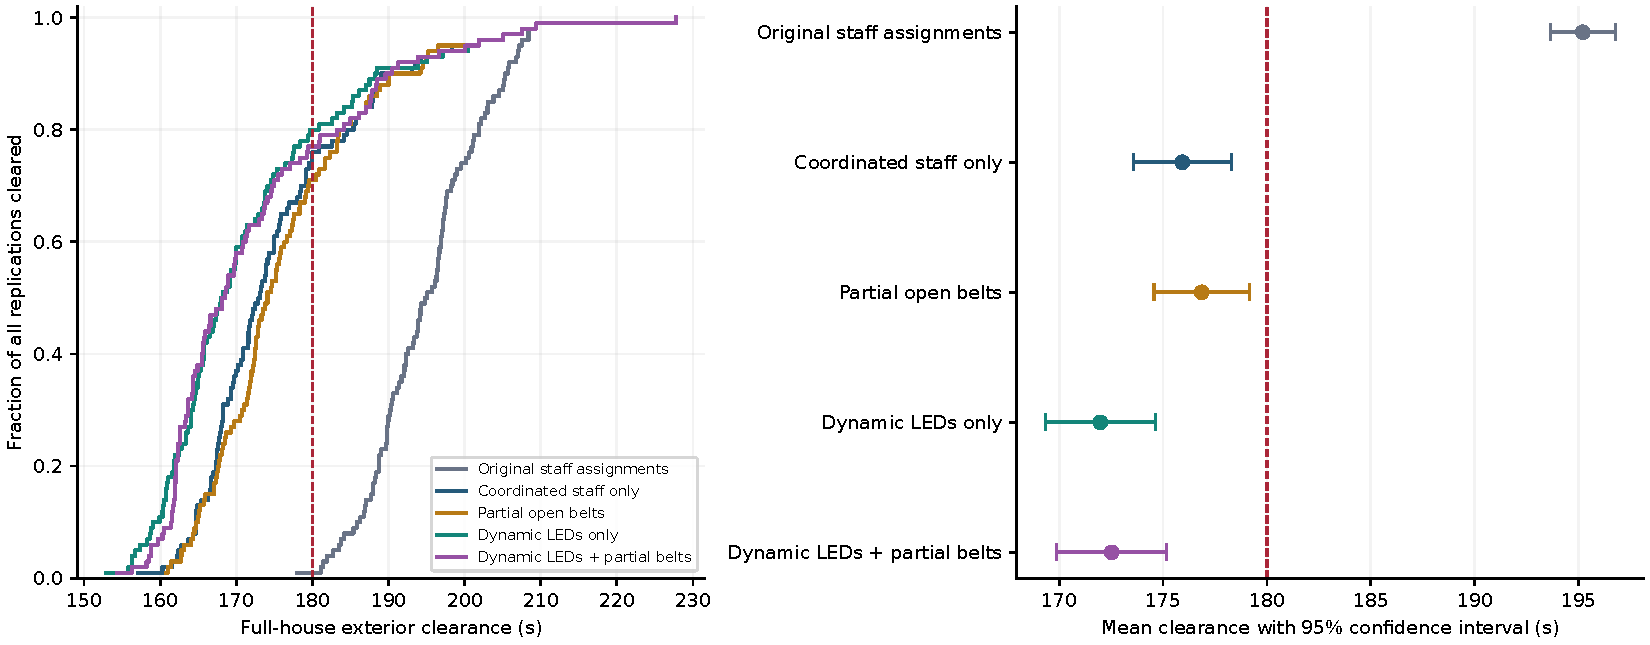
\includegraphics[width=\linewidth]{figures/monte-carlo-comparison.pdf}

\caption{Clearance distributions retain all replications in the denominator. The dashed line marks 180 s. Error bars are 95\% confidence intervals for the mean, not prediction intervals.}\end{figure}

\begin{table}[htbp]\centering\small

\begin{tabular}{lrr}\toprule

Paired contrast & Mean difference (s) & 95\% CI (s)\\\midrule

LED effect without barriers & -3.9 & -6.1 to -1.8\\

Barrier effect without LEDs & 0.9 & -0.2 to 2.1\\

Barrier effect with LEDs & 0.5 & -0.4 to 1.5\\

Combined effect & -3.4 & -5.4 to -1.4\\

\bottomrule\end{tabular}

\caption{Within-seed differences; negative means faster. These isolate interventions from staff coordination and engine corrections.}\end{table}

\begin{figure}[htbp]\centering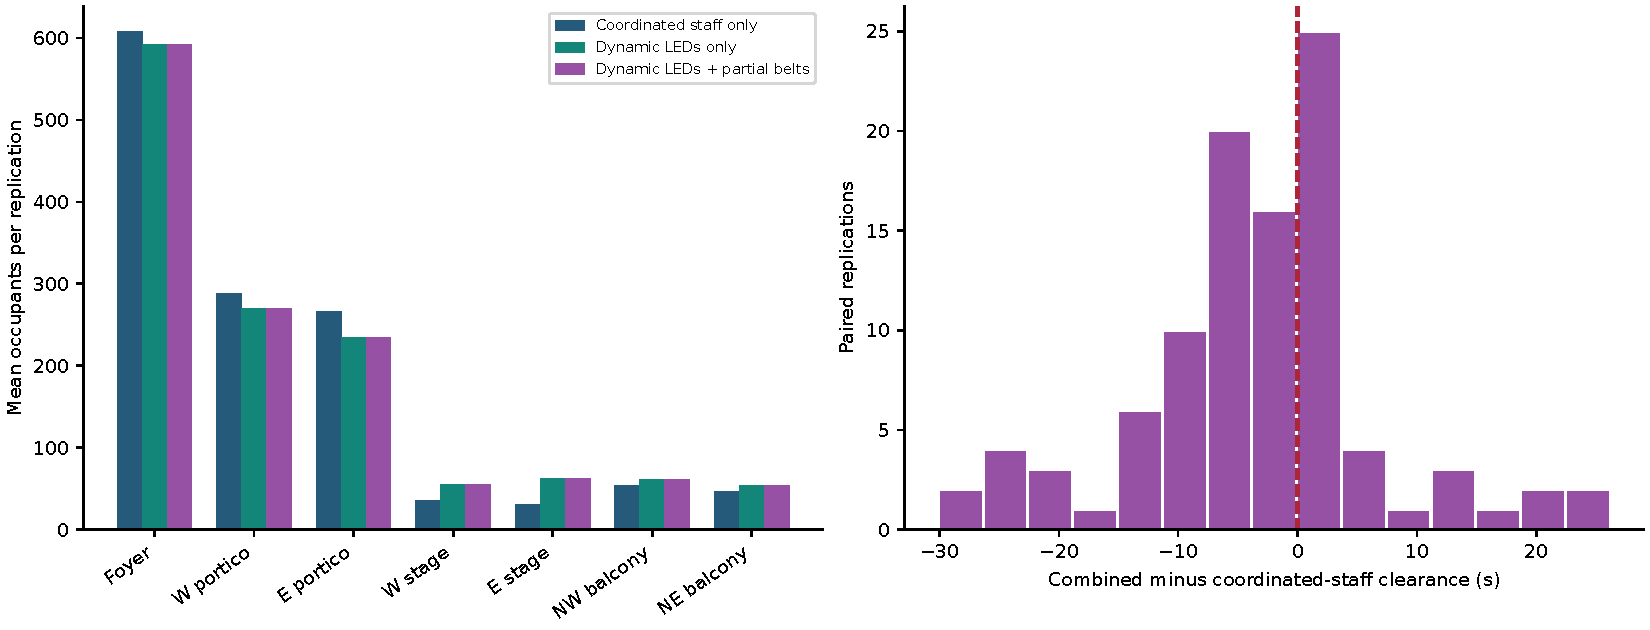
\includegraphics[width=\linewidth]{figures/intervention-effects.pdf}

\caption{Exit redistribution and paired combined-policy differences. No additional door capacity is assigned to guidance or barriers.}\end{figure}

The selected combination evacuated 300/300 wheelchair-user observations across the exterior boundary and 300/300 to street level. The three observations within each replication share the crowd environment. Mean accumulated queue wait was 33.1 s per person. Full logs, policy JSON, source hashes and per-seed results accompany the repository report.

\subsection{Interpretation of the Comparisons}

Changing the six managers' messages changes mean clearance by -19.3 s relative to the original messages. Adding dynamic LEDs to coordinated staff changes it by -3.9 s. These comparisons use the same corrected engine and separate staffing information from the device effects.

Adding partial belts to the LED layout changes mean clearance by 0.5 s (paired 95\% CI -0.4 to 1.5 s). The interval includes zero: the study does not establish an incremental belt benefit, and this is not proof of equivalence.

The slower-response sensitivity and time-step differences must be considered alongside the main result. The 180-second criterion is conditional on the reference audience and prompt response assumptions, not a demonstrated property of the real hall.

\subsection{Numerical Refinement and Sensitivities}

The selected combination was rerun for the first three validation audiences with $\Delta t=0.0125$ s, compared with the prescribed 0.1 s step. Only the integration interval changes. These are numerical checks, not three additional independent validation audiences.

\begin{table}[htbp]\centering\small

\begin{tabular}{rrrr}\toprule

Seed & Coarse clearance (s) & Fine clearance (s) & Fine minus coarse (s)\\\midrule

5001 & 168.9 & 164.8 & -4.1\\

5002 & 168.5 & 187.6 & 19.1\\

5003 & 187.8 & 185.0 & -2.8\\

\bottomrule\end{tabular}\caption{Time-step refinement; full-run invariant and replay checks pass at both steps.}\end{table}

The full network exhibits material numerical sensitivity: route decisions and lane-request ordering can change discontinuously. These three pairs do not establish time-step convergence. Isolated saturated-gate tests verify the prescribed throughput at both intervals, but that does not imply a converged full-house clearance estimate. The 0.1 s reference is retained regardless of whether refinement is faster or slower. Monte Carlo confidence intervals exclude this numerical uncertainty.

Two separately labelled parameter sensitivities use 20 audiences per policy, seeds 6001--6020. The low-guidance case changes staff acceptance from 0.85 to 0.70, LED detection from 0.77 to 0.60, and LED acceptance from 0.80 to 0.60. The slow-response cases use recognition and preparation medians of 10 and 30 s instead of 6 and 14 s. These assumptions are stress cases, not fitted literature estimates. Main-study parameters and layouts remain unchanged.

\begin{table}[htbp]\centering\small

\begin{tabular}{lrrr}\toprule

Case & Complete & Mean (s) & $T\leq180$\\\midrule

Combined, nominal guidance & 20/20 & 175.4 & 13/20\\

Combined, weaker guidance & 20/20 & 175.9 & 12/20\\

Original staff, slower response & 20/20 & 259.1 & 0/20\\

Combined, slower response & 20/20 & 258.8 & 0/20\\

\bottomrule\end{tabular}\caption{Separate parameter sensitivities. A censored case has no unconditional mean.}\end{table}

Weaker guidance minus nominal guidance: paired mean difference 0.5 s over 20 complete pairs. Student-t 95\% interval: -6.8 to 7.8 s.

Combined minus original staff under slower response: paired mean difference -0.3 s over 20 complete pairs. Student-t 95\% interval: -3.4 to 2.8 s.

The slow-response tail is visible in individual records: in seed 6008, the last occupant has a sampled preparation delay of 301.8 s and crosses outside at 352.8 s; in seed 6020 the corresponding delay is 312.9 s and clearance is 349.3 s. These are model draws, not observed people. No response-tail truncation was introduced to force the benchmark, and neither last occupant changes destination after the initial choice in these records.

\subsection{Verification and Reproducibility}

The final implementation passed 49 automated engine tests and 4 browser tests, plus TypeScript and production builds. All 500 confirmatory archives and all 86 numerical/sensitivity archives were audited against hashes and reconstructed crossing counts. Each study exactly replayed the complete first-seed result for every policy. Initial audience hashes confirm distinct audiences across replications and identical paired audiences across policies. Every run enforces population conservation, storage, connectivity and accessibility invariants. These checks establish consistency with the declared model, not empirical validation of Bailey Hall.

